%---------------------------------------------------------------------------%
%->> 封面信息及生成
%---------------------------------------------------------------------------%
%-
%-> 中文封面信息
%-
\confidential{}% 密级：只有涉密论文才填写
\schoollogo{scale=0.2}{ShanghaiTechLogo}% 校徽
%======论文题目 页眉显示 务必准确========
\title{面向动态目标的机械臂模仿学习控制方法研究}% 论文中文题目
\author{唐林峥}% 论文作者
\ID{2022533087}
\entranceYear{2022}
\advisor{白卫邦、马成毓}% 指导教师：姓名
\advisorsec{}% 第二指导老师：按情况填写
\degree{学士}% 学位：学士、硕士、博士
\degreetype{工学}% 学位类别：理学、工学、工程、医学等
\major{计算机科学与技术}% 二级学科专业名称
\institute{信息科学与技术学院}% 院系名称
\chinesedate{2026~年~6~月}% 毕业日期：夏季为6月、冬季为12月
%-
%-> 英文封面信息
%-
\englishtitle{Imitation Learning-Based Control of Robotic Manipulators for Dynamic Targets}% 论文英文题目
\englishauthor{Tang Linzheng}% 论文作者
\englishadvisor{Weibang Bai, Chengyu Ma}% 指导教师
\englishdegree{Bachelor}% 学位：Bachelor, Master, Doctor。封面格式将根据英文学位名称自动切换，请确保拼写准确无误
\englishdegreetype{Engineering}% 学位类别：Philosophy, Natural Science, Engineering, Economics, Agriculture 等
\englishthesistype{thesis}% 论文类型： thesis, dissertation
\englishmajor{Computer Science and Technology}% 二级学科专业名称
\englishinstitute{School of Information Science and Technology}% 院系名称
\englishdate{June, 2026}% 毕业日期：夏季为June、冬季为December
%-
%-> 生成封面
%-
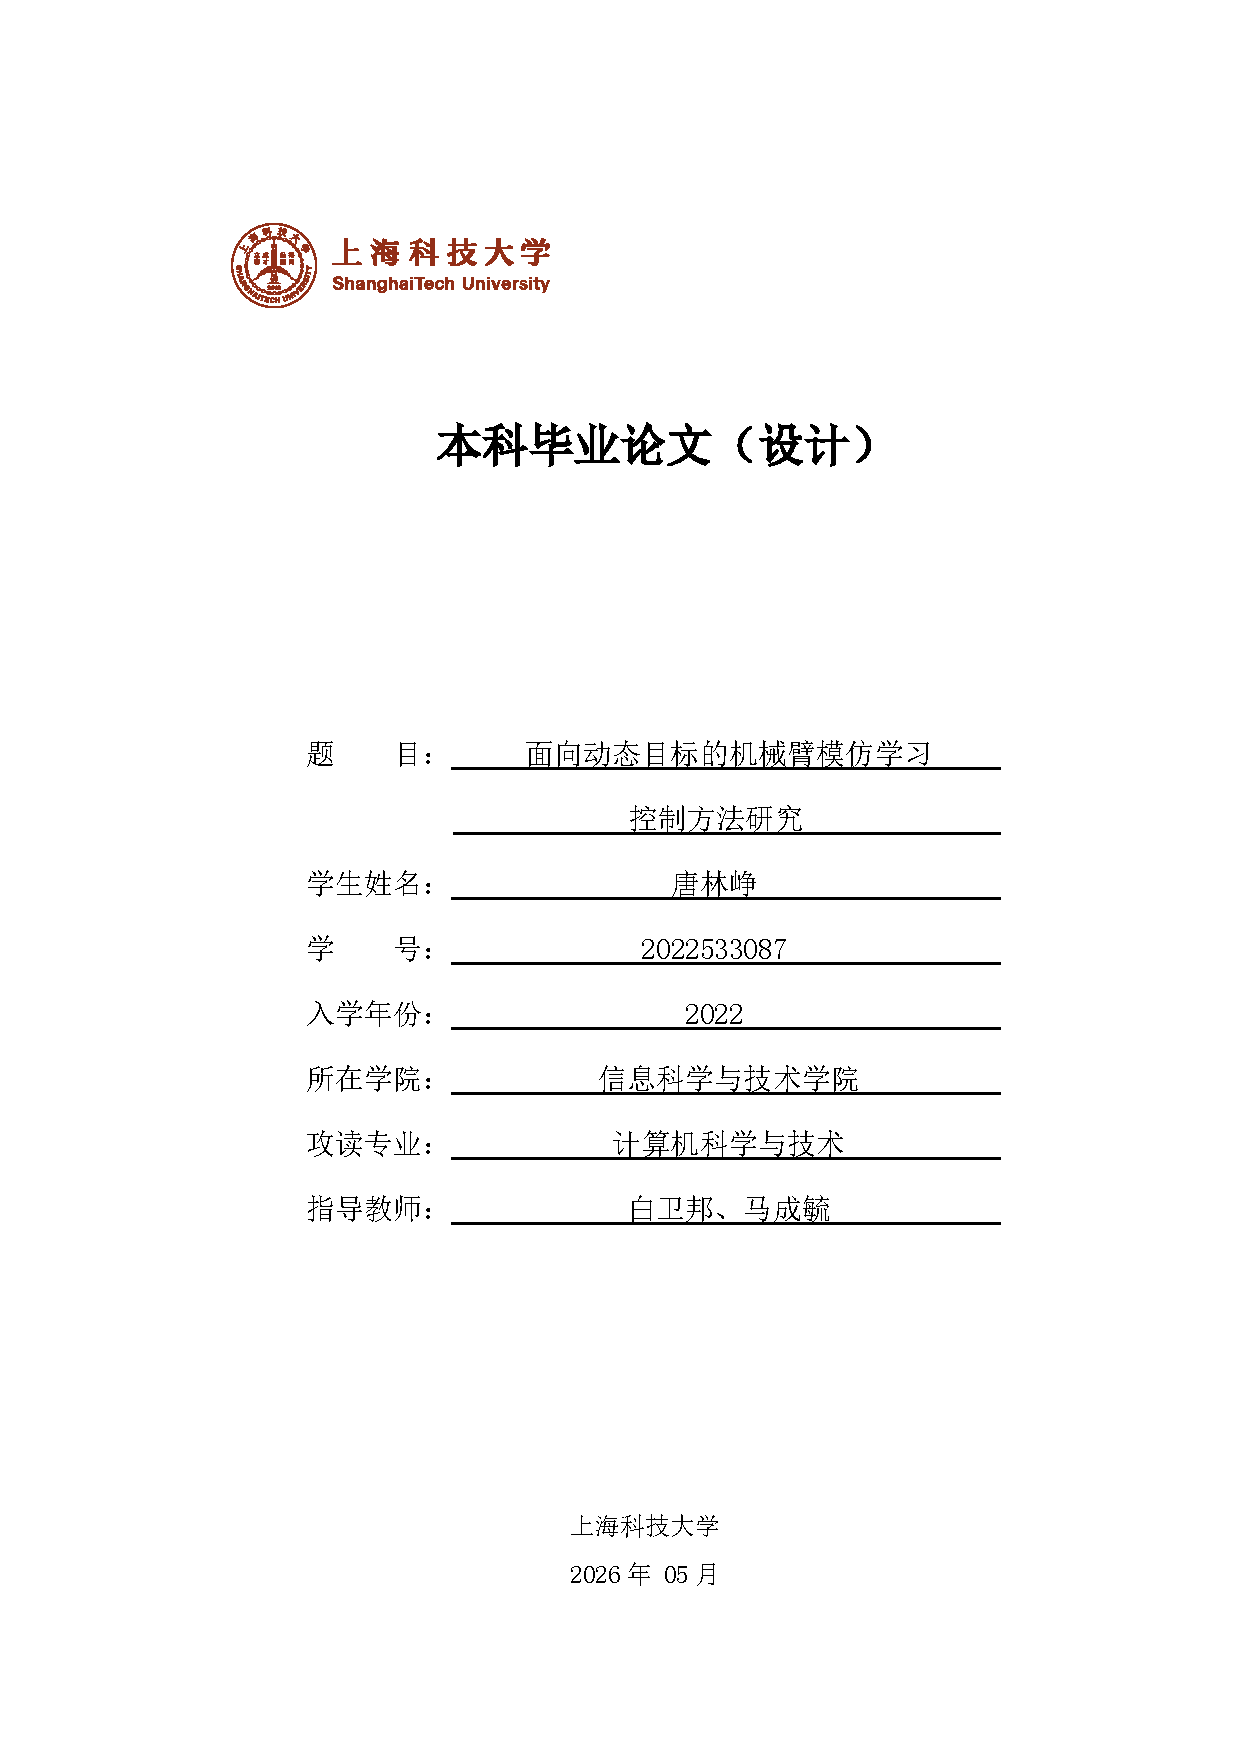
\includepdf[pages=-]{cover.pdf}% 插入预生成的封面PDF（中文+英文）
%-
%-> 作者声明
%-

\includepdf[pages=-]{integrity.pdf}% 插入预生成的诚信书

\includepdf[pages=-]{copyright.pdf}% 插入预生成的版权授权书
%-
%-> 中文摘要
%-
\chapter*{摘\quad 要}\chaptermark{摘\quad 要}% 摘要标题
\setcounter{page}{1}% 开始页码
\pagenumbering{Roman}% 页码符号

动态目标抓取要求机械臂在目标持续平移和旋转时，依次完成接近、相对位姿对齐、夹爪闭合、保持与搬运。与静态抓取或单步轨迹跟踪相比，该任务对运动目标的相对表示、短时历史信息的利用以及闭环时机的判断有较高要求。本文以动态立方体抓取为研究对象，构建目标中心动作块模仿学习框架，并在统一数据、统一动作接口和统一闭环执行协议下比较多类学习策略。研究重点不在于提出单一新模型，而在于分析哪些设计因素真正决定动态目标抓取的闭环成功率。

本文收集了5000条成功专家示教，并在每个主要条件下进行750回合闭环评估，得出了三个主要发现。

第一，目标中心表示是最稳定的性能决定因素。以ACT为例：使用目标中心表示时成功率为57.3\%--59.2\%；切换至世界坐标表示后降至8.8\%--27.2\%，性能差距约30--50个百分点。这一差距明显大于ACT与BC-RNN之间的架构差异（约10个百分点）。

第二，当物体姿态随机变化且伴随平移时，策略需要时间结构和动作块输出。单步BC几乎完全失败（0.1\%），而BC-RNN和ACT分别达到48.7\%和59.2\%。这表明抓取面选择、姿态对齐和闭合时机的判断依赖于历史上下文和多步动作组织。

第三，单纯依靠增加模型容量或更换策略类别并不能保证成功。在本文采用的低维动作空间与10步DDIM条件下，扩散策略（DP）在不同模型容量下的成功率均在1.3\%--2.8\%之间。这表明动态抓取性能主要取决于表示和时间结构，而非模型复杂度。

除表示和时间结构外，感知噪声下的状态估计方式同样影响闭环表现。噪声实验表明，状态估计策略需要与控制器结构适配。专家FSM-MPC控制器在强噪声下完全失效（0.0\%），加入卡尔曼滤波后恢复至56.4\%，说明显式状态估计对基于规则和优化的控制器至关重要。相比之下，ACT和BC-RNN在卡尔曼滤波后的变化仅为$+2.5$和$-5.2$个百分点，表明学习策略依靠历史窗口和动作块结构已自然具备隐式时间平滑能力。综合来看，在FSM-MPC专家示教框架内，动态目标抓取的有效学习控制取决于目标中心表示、时间动作块与状态估计方式三者的协调，而非单纯更换或扩大策略架构。上述发现表明，学习策略的表示设计与经典控制器的状态估计之间存在互补关系，体现了混合控制的基本思路。

\keywords{模仿学习，动作块，动态目标抓取，目标中心表示，混合控制}% 中文关键词
%-
%-> 英文摘要
%-
\chapter*{Abstract}\chaptermark{Abstract}% 摘要标题

Dynamic object grasping requires a manipulator to approach, align with, close on, hold, and transport a target that is continuously moving. Compared with static grasping or one-step trajectory tracking, this task demands accurate relative-motion representation, short-horizon temporal context, and precise timing of gripper closure within the closed loop. This thesis studies dynamic cube grasping through a target-centric action-chunk imitation learning framework, where multiple learned policies are compared under the same demonstration dataset, action interface, and closed-loop execution protocol. The goal is not to propose a new architecture, but to identify which design factors determine closed-loop success in moving-target manipulation.

Based on 5000 successful expert demonstrations and 750 closed-loop evaluation episodes per main condition, the experiments yield three main findings.

First, target-centric representation is the most consistent performance determinant. ACT reaches 57.3--59.2\% success with target-centric state, but drops to 8.8--27.2\% with world-frame state. This gap of roughly 30--50 percentage points far exceeds the architectural difference between ACT and BC-RNN (roughly 10 percentage points).

Second, when the object undergoes arbitrary tumbling and translation, temporal structure and action chunks are essential. One-step BC almost completely fails (0.1\%), whereas BC-RNN and ACT reach 48.7\% and 59.2\% respectively. This indicates that history and multi-step action organization are necessary for grasp-face selection, pose alignment, and gripper closing timing.

Third, model class or capacity alone does not ensure success. Under the low-dimensional action space and 10-step DDIM setup used in this thesis, all DP variants remain in the 1.3--2.8\% success range, suggesting that representation and temporal structure are stronger constraints than model scale in this setting.

The noise experiments further show that state estimation must be aligned with the controller structure. The expert FSM-MPC controller fails completely under strong perceptual noise (0.0\%), but recovers to 56.4\% with a Kalman filter, indicating that explicit state estimation is critical for rule- and optimization-based control. In contrast, ACT and BC-RNN exhibit only modest shifts of +2.5 and -5.2 percentage points with Kalman filtering, suggesting that learned temporal policies already provide inherent smoothing through history windows and action chunks.

Overall, effective learned control for dynamic grasping depends on three coordinated elements: target-centric representation, temporal action chunks, and controller-appropriate state estimation. These design factors, rather than policy architecture scaling, determine success within the FSM-MPC expert demonstration framework. This thesis demonstrates a hybrid control perspective in which learned policies and classical controllers are complementary.

\englishkeywords{Imitation Learning, Action Chunking, Dynamic Grasping, Target-Centric Representation, Hybrid Control}% 英文关键词
%---------------------------------------------------------------------------%
